\documentclass{article}
\usepackage{tikz}
\usepackage{xcolor}
\usetikzlibrary{arrows.meta,positioning,fit,backgrounds,calc,shapes.geometric}

\definecolor{nxgray}{RGB}{120,120,120}
\definecolor{nxblue}{RGB}{0,100,255}
\definecolor{nxred}{RGB}{255,50,50}
\definecolor{nxteal}{RGB}{0,150,150}
\definecolor{nxamber}{RGB}{255,150,0}

\begin{document}
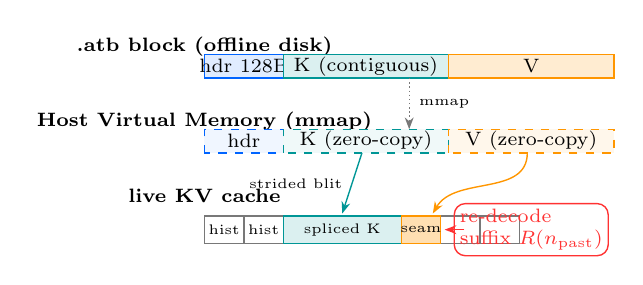
\begin{tikzpicture}[font=\scriptsize,line width=0.5pt]
% .atb block on disk
\node[align=center] at (0,2.5) {\textbf{.atb block (offline disk)}};
\draw[fill=nxblue!12,draw=nxblue] (0,2.1) rectangle (1.0,2.4) node[midway]{hdr 128B};
\draw[fill=nxteal!14,draw=nxteal] (1.0,2.1) rectangle (3.1,2.4) node[midway]{K (contiguous)};
\draw[fill=nxamber!18,draw=nxamber] (3.1,2.1) rectangle (5.2,2.4) node[midway]{V};

% Host Virtual Memory (mmap)
\node[align=center] at (0,1.55) {\textbf{Host Virtual Memory (mmap)}};
\draw[fill=nxblue!6,draw=nxblue,dashed] (0,1.15) rectangle (1.0,1.45) node[midway]{hdr};
\draw[fill=nxteal!6,draw=nxteal,dashed] (1.0,1.15) rectangle (3.1,1.45) node[midway]{K (zero-copy)};
\draw[fill=nxamber!8,draw=nxamber,dashed] (3.1,1.15) rectangle (5.2,1.45) node[midway]{V (zero-copy)};

% live cache
\node[align=center] at (0,0.6) {\textbf{live KV cache}};
\foreach \x in {0,...,7}{\draw[draw=nxgray] (\x*0.5,0.0) rectangle (\x*0.5+0.5,0.35);}
\node at (0.25,0.175){\tiny hist};\node at (0.75,0.175){\tiny hist};
\draw[fill=nxteal!14,draw=nxteal] (1.0,0.0) rectangle (2.5,0.35);
\node at (1.75,0.175){\tiny spliced K};
\draw[fill=nxamber!30,draw=nxamber] (2.5,0.0) rectangle (3.0,0.35);
\node at (2.75,0.175){\tiny seam};

% arrows
\draw[-{Stealth[length=1.5mm]},draw=nxgray,densely dotted] (2.6,2.1) -- (2.6,1.45) node[midway,right]{\tiny mmap};
\draw[-{Stealth[length=1.5mm]},draw=nxteal] (2.0,1.15) -- (1.75,0.38) node[midway,left]{\tiny strided blit};
\draw[-{Stealth[length=1.5mm]},draw=nxamber] (4.1,1.15) to[out=-90,in=60] (2.9,0.38);
\node[align=left,draw=nxred,rounded corners,inner sep=2pt,text=nxred] at (4.15,0.175)
  {re-decode\\suffix $R(n_{\mathrm{past}})$};
\draw[-{Stealth[length=1.5mm]},draw=nxred] (3.3,0.175) -- (3.05,0.175);
\end{tikzpicture}
\end{document}
